% Provenance (never printed): enseignement scientifique premiere (2019),
% "Le Soleil, notre source d'energie" (power received by latitude and
% season, albedo, the Earth's radiative balance, the small share stored by
% photosynthesis) and the old seconde/premiere S material on the
% atmosphere's energy; see sources/book2/PROVENANCE.md. Every insolation
% value, budget closure and photosynthesis figure is computed in
% figdata/grade-10/energy_budget.py; the budget fluxes are AR6 WG1
% Figure 7.2.
\chapter{पृथ्वी का ऊर्जा बजट}\label{ch:g10:earth-energy-budget}

वर्ष के सबसे लंबे दिन उत्तरी ध्रुव पर सूर्य अस्त ही नहीं होता। वह पूरे दिन क्षितिज से लगभग
\qty{23}{\degree} की एक ही ऊँचाई पर आकाश का चक्कर लगाता है, और ध्रुव के ऊपर
वायुमंडल का शीर्ष एक दिन में प्रति वर्ग मीटर पृथ्वी पर किसी भी अन्य स्थान से अधिक
सूर्य-प्रकाश पाता है --- \qty{13.0}{kWh}, जबकि भूमध्य रेखा के ऊपर \qty{9.5}{kWh}। फिर भी
ध्रुव के चारों ओर का समुद्र पूरी गर्मियों में बर्फ़ से ढका रहता है। दूसरी ओर, पूरे वर्ष में
भूमध्य रेखा ध्रुव की तुलना में ढाई गुना सूर्य-प्रकाश पाती है, और उष्णकटिबंध पूरे वर्ष गरम
रहते हैं। यह अध्याय सूर्य-प्रकाश की ऊर्जा का अनुसरण करता है: कितनी आती है, कहाँ और कब;
कितनी सीधे अंतरिक्ष में लौटा दी जाती है; बाक़ी हवा और ज़मीन के बीच कैसे बँटती है, उष्णकटिबंध
से ध्रुवों की ओर कैसे ले जाई जाती है, और अंत में अवरक्त प्रकाश के रूप में अंतरिक्ष में कैसे
वापस भेजी जाती है --- और उसका कौन-सा नन्हा-सा भाग जीवों में संचित होता है।
% ledger: earth:TSI, earth:obliquity (daily totals computed in figdata/grade-10/energy_budget.py)

\begin{omfigure}
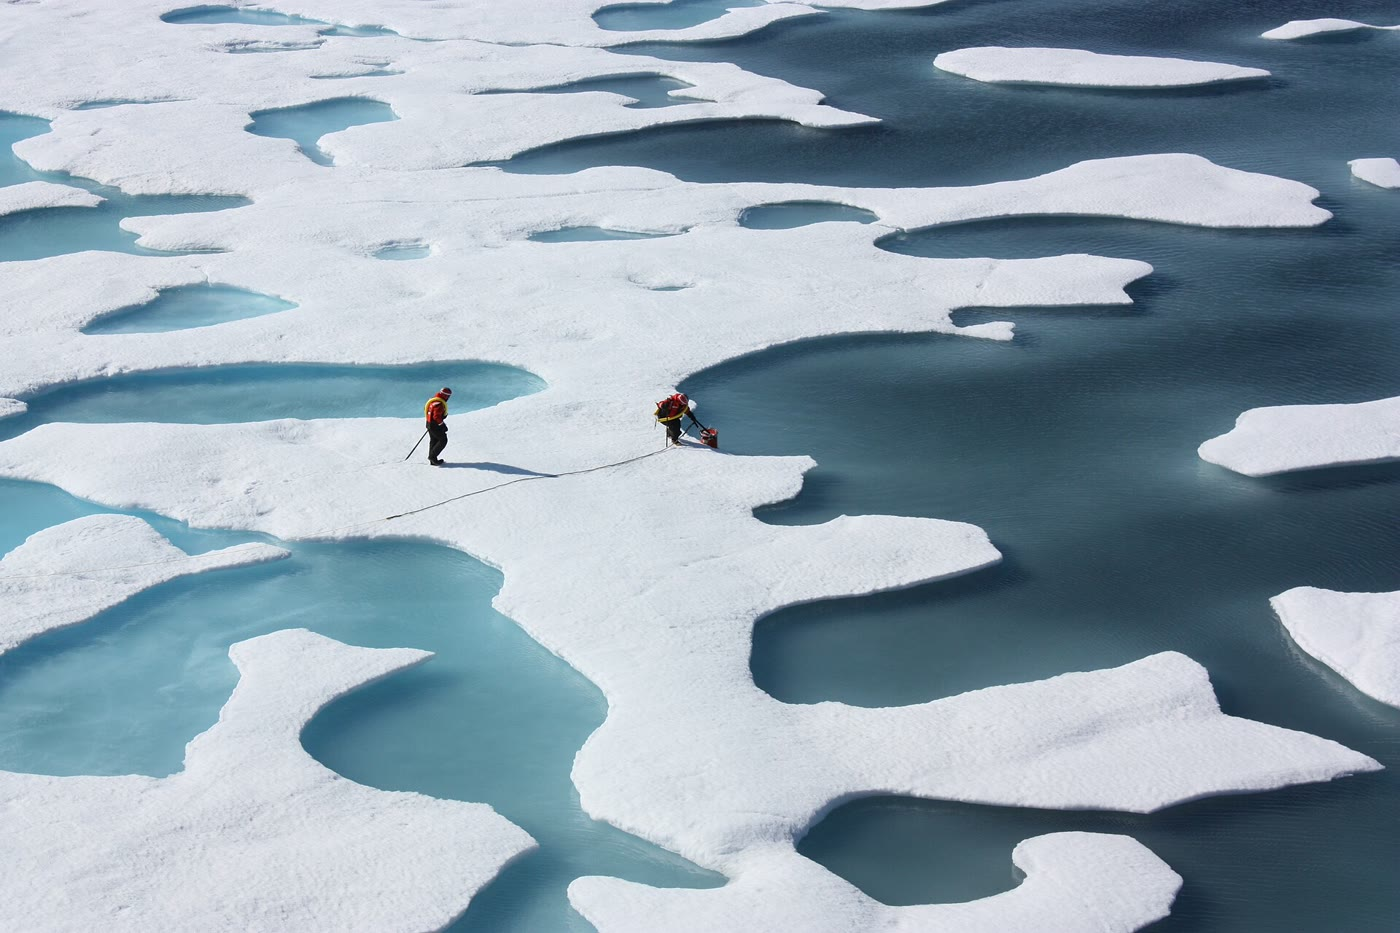
\includegraphics[width=0.78\linewidth]{images/book2/g10-nasa-melt-ponds.jpg}

{\small जुलाई में आर्कटिक महासागर की समुद्री बर्फ़, कभी न डूबने वाले सूर्य के नीचे: सफ़ेद बर्फ़,
उसकी सतह पर पिघले जल के ताल, और हिम-खंडों के बीच गहरे रंग का खुला समुद्र। दो वैज्ञानिक
तालों के नमूने ले रहे हैं। फ़ोटो: NASA गोडार्ड
स्पेस फ़्लाइट सेंटर, 2011 (सार्वजनिक डोमेन)।}
\end{omfigure}

\begin{recall}
ऋतुएँ पृथ्वी के अक्ष के झुकाव से आती हैं, जो उसकी कक्षा के तल के लंब से \qty{23.44}{\degree}
झुका है: जून में उत्तरी गोलार्ध सूर्य की ओर झुका होता है, जो उसके आकाश में ऊँचा चढ़ता है और
देर तक ऊपर रहता है (भौतिकी की पुस्तकें, और पुस्तक 1)। पृथ्वी की दूरी पर किरणन,
$S_0 = \qty{1361}{W/m^2}$, किसी ग्रह का बॉन्ड \omterm{def:g10:earth-energy-budget:albedo}{एल्बिडो} और उसका \omterm{def:g10:habitable-planet:equilibrium-temperature}{साम्य तापमान}
\cref{ch:g10:habitable-planet} में आ चुके हैं।
ग्रीनहाउस गैसें सतह द्वारा उत्सर्जित अवरक्त का एक भाग अवशोषित करती हैं (रसायन विज्ञान
की पुस्तकें)। गरम हवा ऊपर उठती है और ठंडी हवा नीचे बैठती है, जिससे हवा संवहन कोष्ठों में
घूमने लगती है और वैश्विक पवनें चलती हैं (पुस्तक 1, कक्षा 8)।
पौधे, शैवाल और कुछ जीवाणु प्रकाश की ऊर्जा से कार्बन डाइऑक्साइड और जल से शर्कराएँ बनाते
हैं: प्रकाशसंश्लेषण (जीव विज्ञान की पुस्तकें)।
\end{recall}

\section{प्राप्त सूर्य-प्रकाश}

सूर्य से देखने पर पृथ्वी एक चकती है। हर सेकंड वह उस सूर्य-प्रकाश को रोकती है जो
त्रिज्या $R$, यानी उसकी अपनी त्रिज्या, की चकती पर पड़ता है; पर वह प्रकाश एक गोले के सभी
बिंदुओं में बँटता है, जिनमें से आधे रात में होते हैं।

\begin{proposition}[सौर नियतांक का एक-चौथाई]\label{prop:g10:earth-energy-budget:quarter}
पृथ्वी की पूरी सतह पर और दिन तथा रात पर औसत लेने पर, वायुमंडल के शीर्ष पर पहुँचने वाले
सूर्य-प्रकाश की शक्ति है
\[
  \frac{S_0}{4} = \frac{1361}{4} \approx \qty{340}{W/m^2}.
\]
\end{proposition}

\begin{proof}
पृथ्वी उस सूर्य-प्रकाश को रोकती है जो किरणों के लंबवत क्षेत्रफल $\pi R^2$ की
चकती को पार करता है, यानी शक्ति $S_0\,\pi R^2$। गोले के
क्षेत्रफल, $4\pi R^2$, पर फैलाने से प्रति वर्ग मीटर $S_0\,\pi R^2/(4\pi R^2) =
S_0/4$ मिलता है।
\end{proof}
% ledger: earth:TSI, ipcc:budget-toa

\begin{omfigure}
\begin{tikzpicture}[font=\small, >={Stealth[length=2mm]}]
  \foreach \y in {-1.2,-0.8,...,1.21}
    \draw[->, omProp!80!black] (-3.4,\y) -- (-1.75,\y);
  \node[anchor=south, font=\footnotesize, align=center] at (-2.6,1.35) {सूर्य-प्रकाश,\\$S_0$ प्रति m$^2$};
  \draw[fill=omProp!15, draw=omProp!80!black] (-1.6,0) ellipse (0.18 and 1.3);
  \node[anchor=north, font=\footnotesize, align=center] at (-1.6,-1.4) {चकती\\$\pi R^2$};
  \shade[ball color=omDef!35] (1.2,0) circle (1.3);
  \fill[black, opacity=0.35] (1.2,1.3) arc (90:-90:1.3) arc (-90:90:0.35 and 1.3);
  \draw[omDef!80!black] (1.2,0) circle (1.3);
  \draw[dashed, black!50] (1.2,-1.3) arc (-90:90:0.35 and 1.3);
  \draw[<->] (1.2,0) -- node[above, font=\footnotesize] {$R$} (2.5,0);
  \node[anchor=west, font=\footnotesize, align=left] at (2.8,0.7) {गोला $4\pi R^2$:\\आधा दिन के प्रकाश में,\\आधा रात में};
  \node[anchor=west, font=\footnotesize, align=left] at (2.8,-0.75) {औसत:\\$S_0\pi R^2/4\pi R^2 = S_0/4$};
\end{tikzpicture}

{\small पृथ्वी उस सूर्य-प्रकाश को रोकती है जो उसकी अपनी त्रिज्या की चकती पर पड़ता है, पर उसे
गोले के चार गुना बड़े क्षेत्रफल में बाँट देती है: औसतन वायुमंडल के शीर्ष का हर वर्ग मीटर
सौर नियतांक का एक-चौथाई पाता है।}
\end{omfigure}

यह औसत स्थान-स्थान के बड़े अंतरों को छिपा लेता है। तिरछा होकर ज़मीन से टकराने वाला
सूर्य-प्रकाश का पुंज सीधे टकराने वाले पुंज की तुलना में अधिक बड़े क्षेत्रफल पर फैलता है।

\begin{proposition}[क्षैतिज सतह पर सूर्य-प्रकाश]\label{prop:g10:earth-energy-budget:height}
जब सूर्य क्षितिज से ऊँचाई $h$ पर हो, तो वायुमंडल के शीर्ष पर एक क्षैतिज वर्ग मीटर
शक्ति $S_0 \sin h$ पाता है।
\end{proposition}

\begin{proof}
\qty{1}{m^2} अनुप्रस्थ काट वाला एक वर्गाकार सूर्य-प्रकाश पुंज लीजिए, जो
$S_0$ ले जाता है। ज़मीन पर उसका चिह्न एक आयत है, जिसकी एक भुजा \qty{1}{m} की है
और दूसरी, किरणों के ढलान के अनुदिश, लंबाई $\ell$ की। उस भुजा, किरण और पुंज की
अनुप्रस्थ काट से बने समकोण त्रिभुज में ज़मीन पर का कोण $h$ है और $\sin h = 1/\ell$।
पुंज की शक्ति $\ell$ वर्ग मीटरों पर फैल जाती है: प्रति वर्ग
मीटर $S_0/\ell = S_0 \sin h$।
\end{proof}

\begin{omfigure}
\begin{tikzpicture}[font=\small, >={Stealth[length=2mm]}]
  \fill[omExo!15] (-0.3,-0.5) rectangle (6.3,0);
  \draw[thick] (-0.3,0) -- (6.3,0);
  \foreach \s in {0,0.3,...,1.21}
    \draw[->, omProp!80!black] ({0.6+\s/sin(35)+3.2*cos(35)},{3.2*sin(35)}) -- ({0.6+\s/sin(35)+0.02*cos(35)},{0.02*sin(35)});
  \draw[omProp!80!black, thick] (0.6,0) -- ({0.6+1.2/sin(35)},0);
  \draw (0.6,0) ++(1.6,0) arc (0:35:1.6);
  \node[font=\footnotesize] at ({0.6+1.85*cos(17)},{1.85*sin(17)}) {$h$};
  \draw[<->] (0.6,-0.25) -- node[below, font=\footnotesize] {$\ell = 1/\sin h$} ({0.6+1.2/sin(35)},-0.25);
  \node[anchor=south west, font=\footnotesize, align=left] at (4.35,1.95) {पुंज, जिसकी\\अनुप्रस्थ काट\\\qty{1}{m^2}};
\end{tikzpicture}

{\small क्षितिज से ऊँचाई $h$ पर से आता सूर्य-प्रकाश: वही पुंज
क्षैतिज ज़मीन के $1/\sin h$ वर्ग मीटर ढकता है, इसलिए हर वर्ग मीटर
$S_0 \sin h$ पाता है। सूर्य जितना नीचा, ज़मीन पर सूर्य-प्रकाश उतना ही
दुर्बल।}
\end{omfigure}

सूर्य की ऊँचाई दिन भर बदलती है, और दिन की लंबाई ऋतुओं के साथ बदलती है; किसी स्थान को
मिलने वाली ऊर्जा में दोनों की गिनती होती है।

\begin{definition}[सूर्यातप]\label{def:g10:earth-energy-budget:insolation}
किसी स्थान का \emph{सूर्यातप}\index{सूर्यातप} उसके ऊपर वायुमंडल के शीर्ष पर एक
क्षैतिज वर्ग मीटर द्वारा प्राप्त सूर्य-प्रकाश की शक्ति है। एक दिन के चौबीस घंटों पर औसत
लेने पर वह \emph{दैनिक माध्य
सूर्यातप} है; एक वर्ष पर औसत लेने पर \emph{वार्षिक माध्य सूर्यातप}; दोनों
\unit{W/m^2} में मापे जाते हैं।
\end{definition}

दैनिक माध्य निकालने के लिए दिन के हर क्षण सूर्य की ऊँचाई चाहिए, जिसमें इस पुस्तक से
आगे का गणित लगता है; नीचे के वक्र खींचने वाले कंप्यूटर ने यही किया। दो स्थितियाँ सरल
हैं। विषुव के दिन भूमध्य रेखा पर सूर्य ठीक पूर्व में उगता है, दोपहर को सिर के ऊपर से गुज़रता है
और बारह घंटे बाद ठीक पश्चिम में अस्त होता है; चौबीस घंटों पर औसत लेने से
$S_0/\pi \approx \qty{433}{W/m^2}$ मिलता है (स्वीकृत)। उत्तरी ध्रुव पर
सूर्य बस एक स्थिर ऊँचाई पर आकाश का चक्कर लगाता है, जिसका उपयोग अगला उदाहरण
करता है।

\begin{example}[जून में ध्रुव]\label{ex:g10:earth-energy-budget:pole}
% ledger: earth:TSI, earth:obliquity (values computed in figdata/grade-10/energy_budget.py)
जून अयनांत पर सूर्य पूरे दिन उत्तरी ध्रुव के क्षितिज से \qty{23.44}{\degree} ऊपर
रहता है। वहाँ दैनिक माध्य \omterm{def:g10:earth-energy-budget:insolation}{सूर्यातप} $1361
\times \sin 23.44^\circ \approx \qty{541}{W/m^2}$ है; चौबीस घंटों में
यह $541 \times 24 \approx \qty{13000}{Wh}$ है, यानी प्रति वर्ग मीटर \qty{13.0}{kWh}।
उसी दिन भूमध्य रेखा को
\qty{397}{W/m^2} का दैनिक माध्य मिलता है, यानी प्रति वर्ग मीटर \qty{9.5}{kWh}: वहाँ
दोपहर को सूर्य अधिक ऊँचा चढ़ता है, पर वह बारह घंटे क्षितिज के नीचे रहता है।
\end{example}

\begin{omfigure}
\begin{tikzpicture}
\begin{axis}[omrecord, width=0.92\linewidth, height=6.4cm, xmin=1, xmax=365,
  ymin=0, ymax=600, ylabel={दैनिक माध्य सूर्यातप (\unit{W/m^2})},
  xtick={1,32,60,91,121,152,182,213,244,274,305,335},
  xticklabels={1,2,3,4,5,6,7,8,9,10,11,12}, xlabel={महीना},
  legend style={at={(0.5,1.02)}, anchor=south, legend columns=4, font=\footnotesize, draw=none},
  tick label style={font=\small}, label style={font=\small}]
\addplot[omThm!85!black, thick] table[x=day, y=Q0] {figdata/out/grade-10-energy_budget-daily.dat};
\addlegendentry{भूमध्य रेखा}
\addplot[omProp!90!black, thick, densely dashed] table[x=day, y=Q30] {figdata/out/grade-10-energy_budget-daily.dat};
\addlegendentry{\qty{30}{\degree} उ}
\addplot[omMeth!85!black, thick, dashdotted] table[x=day, y=Q60] {figdata/out/grade-10-energy_budget-daily.dat};
\addlegendentry{\qty{60}{\degree} उ}
\addplot[omDef!85!black, thick] table[x=day, y=Q90] {figdata/out/grade-10-energy_budget-daily.dat};
\addlegendentry{उत्तरी ध्रुव}
\end{axis}
\end{tikzpicture}

{\small उत्तरी गोलार्ध के चार अक्षांशों पर वर्ष भर वायुमंडल के शीर्ष पर दैनिक माध्य \omterm{def:g10:earth-energy-budget:insolation}{सूर्यातप}
(वृत्ताकार कक्षा के लिए, सौर नियतांक और अक्ष के झुकाव से परिकलित)। ध्रुव
आधे वर्ष कुछ नहीं पाता, और जून अयनांत के आसपास किसी भी अन्य स्थान से अधिक पाता है।}
\end{omfigure}

\begin{remark}[वक्रों को पढ़ना]\label{rem:g10:earth-energy-budget:curves}
भूमध्य रेखा का \omterm{def:g10:earth-energy-budget:insolation}{सूर्यातप} लगभग नहीं बदलता: विषुवों पर दो उथले उच्चिष्ठ, जब सूर्य
दोपहर को सिर के ऊपर से गुज़रता है। जितना उत्तर की ओर जाएँ, गर्मी और सर्दी के बीच का
उतार-चढ़ाव उतना ही बड़ा। $90^\circ - 23.44^\circ = \qty{66.56}{\degree}$ से ध्रुव की
ओर दिसंबर अयनांत पर सूर्य क्षितिज के नीचे ही रहता है: ध्रुवीय रात्रि। लगभग 10 मई से
जुलाई के अंत तक उत्तरी ध्रुव और अक्षांश \qty{60}{\degree} उत्तर दोनों भूमध्य रेखा से अधिक
पाते हैं।
\end{remark}

पूरे वर्ष पर चित्र बदल जाता है: वार्षिक माध्य \omterm{def:g10:earth-energy-budget:insolation}{सूर्यातप}, जो नीचे अधिशेष और घाटे वाले अनुभाग
में आलेखित है, भूमध्य रेखा पर \qty{416}{W/m^2} से घटकर
ध्रुवों पर \qty{172}{W/m^2} रह जाता है। ध्रुवीय क्षेत्रों की गर्मियों की प्रचुरता उनकी लंबी
रात और उनके नीचे सूर्य की भरपाई नहीं कर पाती।

\begin{remark}[सूर्य से दूरी ऋतुएँ नहीं बनाती]\label{rem:g10:earth-energy-budget:distance}
% ledger: earth:peri, earth:aph, nasa:earth-perihelion-longitude (ratios computed)
पृथ्वी की कक्षा पूरी तरह वृत्त नहीं है: सूर्य से उसकी दूरी
\num{147.1} और \num{152.1} मिलियन किलोमीटर के बीच, लगभग
\qty{3}{\percent}, बदलती है, इसलिए सूर्य-प्रकाश लगभग \qty{7}{\percent} बदलता है।
पृथ्वी जनवरी के आरंभ में, उत्तरी सर्दी के बीचोंबीच, सूर्य के सबसे निकट होती है। ऊपर के वक्र
इस छोटे परिवर्तन की उपेक्षा करते हैं; ऋतुएँ अक्ष के झुकाव से आती हैं, और दोनों गोलार्धों में
उलटी होती हैं।
\end{remark}

\section{एल्बिडो}

पृथ्वी तक पहुँचने वाले सूर्य-प्रकाश का एक भाग कभी किसी चीज़ को गरम नहीं करता: बादल, हवा,
हिम और समुद्र उसे अंतरिक्ष में लौटा देते हैं।

\begin{definition}[एल्बिडो]\label{def:g10:earth-energy-budget:albedo}
किसी सतह का \emph{एल्बिडो}\index{एल्बिडो} उस पर पड़ने वाले सूर्य-प्रकाश का वह भाग है
जिसे वह परावर्तित करती है, 0 (सारा प्रकाश अवशोषित) और 1 (सारा परावर्तित) के बीच
की एक संख्या। \cref{ch:g10:habitable-planet} का बॉन्ड एल्बिडो
किसी ग्रह का समग्र रूप से लिया गया एल्बिडो है।
\end{definition}

\begin{omfigure}
\begin{tikzpicture}[font=\small, x=9cm, y=0.55cm]
  \foreach \lab/\lo/\hi/\n in {ताज़ा हिम/0.80/0.90/8, समुद्री बर्फ़/0.50/0.70/7,
      मरुस्थली रेत/0.40/0.40/6, पूरी पृथ्वी/0.30/0.30/5, हरी घास/0.25/0.25/4,
      नंगी मिट्टी/0.17/0.17/3, शंकुधारी वन/0.08/0.15/2, खुला महासागर/0.06/0.06/1,
      नया डामर/0.04/0.04/0} {
    \fill[omDef!45] (0,\n-0.32) rectangle (\lo,\n+0.32);
    \ifdim\hi pt>\lo pt
      \fill[omDef!18] (\lo,\n-0.32) rectangle (\hi,\n+0.32);
      \draw[omDef!80!black] (\lo,\n-0.32) rectangle (\hi,\n+0.32);
    \fi
    \draw[omDef!80!black] (0,\n-0.32) rectangle (\lo,\n+0.32);
    \node[anchor=east, font=\footnotesize] at (-0.01,\n) {\lab};
  }
  \draw (0,-0.6) -- (1,-0.6);
  \foreach \x in {0,0.2,...,1.01}
    \draw (\x,-0.6) -- (\x,-0.75) node[below, font=\footnotesize] {\pgfmathprintnumber[fixed, precision=1]{\x}};
  \node[font=\footnotesize] at (0.5,-2.0) {एल्बिडो};
\end{tikzpicture}

{\small सतहों के और समग्र पृथ्वी के विशिष्ट \omterm{def:g10:earth-energy-budget:albedo}{एल्बिडो}; दंड का हल्का भाग सामान्य परास है।
आँकड़े: यूनिवर्सिटी ऑफ़ कोलोराडो बोल्डर,
MOSAiC अभियान; नेशनल स्नो ऐंड आइस डेटा सेंटर।}
\end{omfigure}
% ledger: albedo:surfaces, nsidc:albedo-ice

ताज़ा हिम उस पर पड़ने वाले प्रकाश का अधिकांश लौटा देता है, खुला महासागर लगभग कुछ भी नहीं।
इसी कारण आरंभिक फ़ोटो की समुद्री बर्फ़ ध्रुवीय गर्मियों में भी अपनी ठंडक बनाए रखती है:
उसके ऊपर का हिम सूर्य-प्रकाश का नौ-दसवाँ भाग तक परावर्तित करता है, जबकि हिम-खंडों के
बीच का गहरे रंग का जल उसका लगभग 94 प्रतिशत अवशोषित करता है।
जब बर्फ़ पिघलती है, तो गहरे रंग का जल उसकी जगह ले लेता है और अधिक सूर्य-प्रकाश अवशोषित
करता है, जो और बर्फ़ पिघलाता है: एक स्व-प्रबलक चक्र, जिसे \cref{ch:g12:climate-change}
जलवायु के पुनर्निवेशों के बीच तौलता है।

\begin{omfigure}
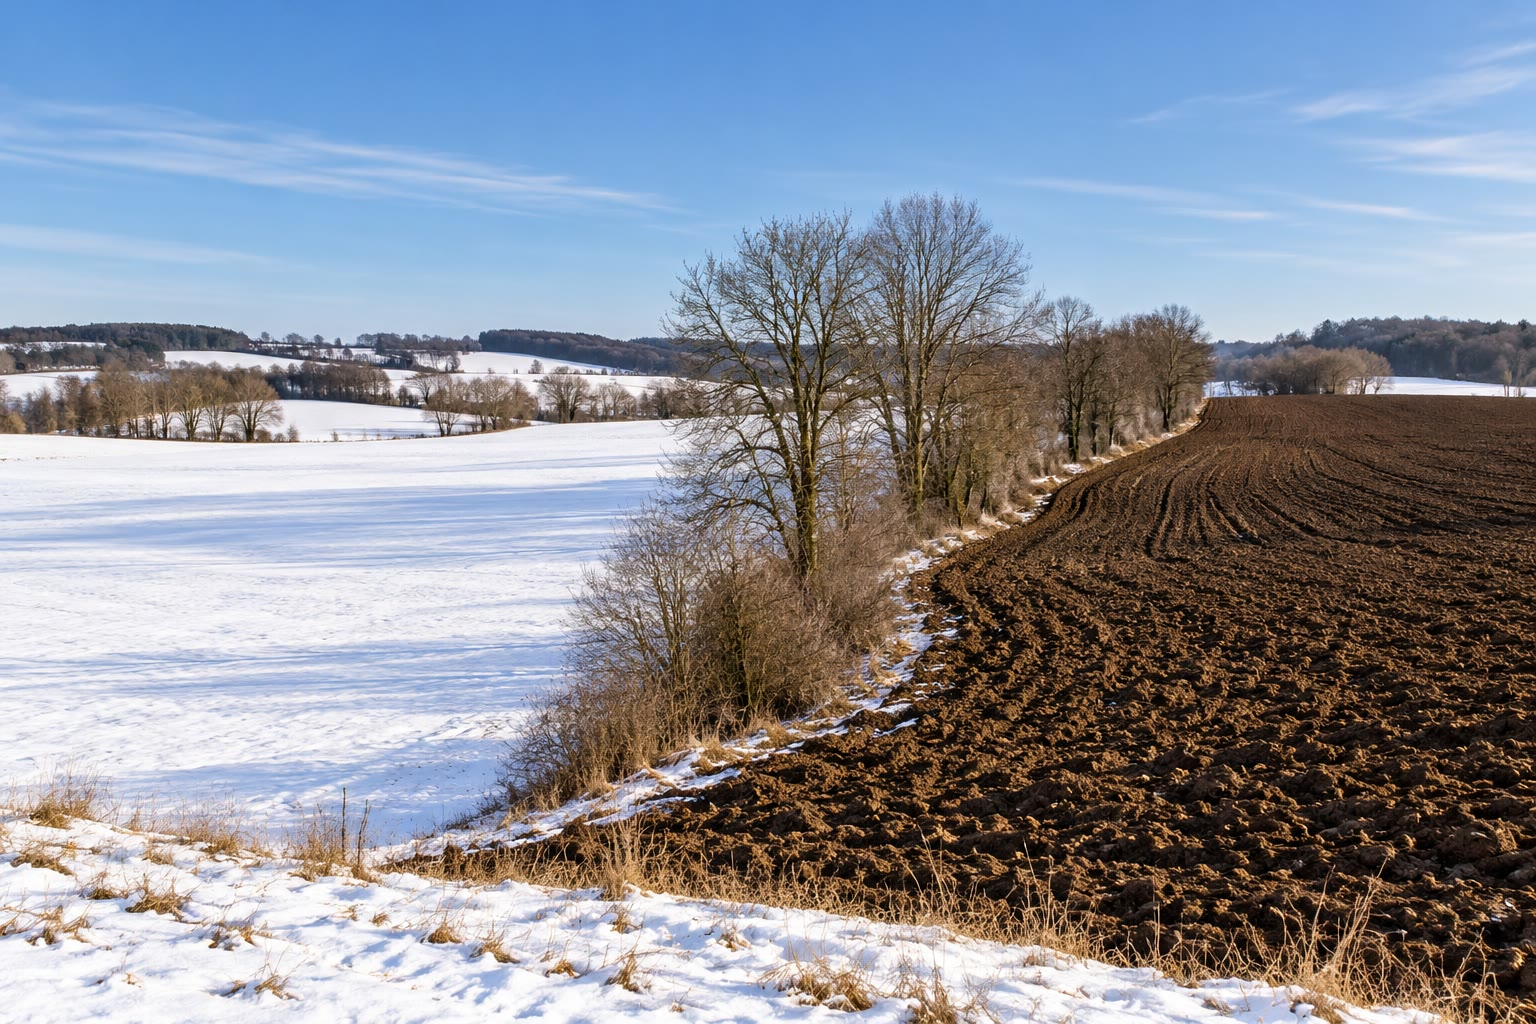
\includegraphics[width=0.7\linewidth]{images/book2/ai/g10-snow-and-ploughed-field.jpg}

{\small कुछ धूप भरे दिनों के बाद सर्दियों की एक सुबह: घास के मैदान पर हिम अब भी पड़ा है, पर
गहरे रंग के जुते हुए खेत पर वह पिघल चुका है, जो सूर्य-प्रकाश का कहीं अधिक भाग
अवशोषित करता है।}
\end{omfigure}

समग्र पृथ्वी के लिए उपग्रह अंतरिक्ष में परावर्तित सूर्य-प्रकाश को सीधे मापते हैं: आने वाले
\qty{340}{W/m^2} में से औसतन \qty{100}{W/m^2},
यानी $100/340 \approx 0.29$ का \omterm{def:g10:earth-energy-budget:albedo}{एल्बिडो}। बादल मुख्य परावर्तक हैं:
उन्हीं मापनों से, बादलों को गणना द्वारा हटाने पर, केवल
\qty{53}{W/m^2} परावर्तित होता है।
% ledger: ipcc:budget-toa, ipcc:budget-clearsky, earth:albedo

\begin{example}[पृथ्वी द्वारा अवशोषित सूर्य-प्रकाश]\label{ex:g10:earth-energy-budget:absorbed}
% ledger: earth:TSI, earth:albedo, earth:Rmean (computed in figdata/grade-10/energy_budget.py)
0.294 के बॉन्ड \omterm{def:g10:earth-energy-budget:albedo}{एल्बिडो} के साथ हर वर्ग मीटर औसतन $340
\times (1 - 0.294) \approx \qty{240}{W/m^2}$ अवशोषित करता है। पूरे गोले पर, जिसका
क्षेत्रफल $4\pi R^2 = 4\pi \times (\qty{6.371e6}{m})^2 \approx \qty{5.10e14}{m^2}$ है,
पृथ्वी $240 \times 5.10\times10^{14} \approx \qty{1.22e17}{W}$
सूर्य-प्रकाश अवशोषित करती है: यही शक्ति पवनों, महासागरीय धाराओं और जल
चक्र को चलाती है।
\end{example}

\section{वैश्विक ऊर्जा बजट}

ये \qty{240}{W/m^2} कहाँ जाते हैं? उपग्रहों, ज़मीन पर रखे उपकरणों और जहाज़ों के मापन,
वायुमंडल के मॉडलों के साथ मिलाकर, अब पूरे ग्लोब पर और कई वर्षों पर औसत किया गया एक
संगत उत्तर देते हैं। 2021 का वैज्ञानिक आकलन इसे नीचे के आरेख में संक्षेप में रखता है, और
कहता है कि वायुमंडल के शीर्ष पर और सतह पर वैश्विक माध्य घटक अब अधिक सटीकता से ज्ञात
हैं (\emph{उच्च
विश्वास})।
% ledger: ipcc:budget-confidence

\begin{definition}[ऊर्जा बजट]\label{def:g10:earth-energy-budget:energy-budget}
किसी तंत्र --- पूरी पृथ्वी, उसकी सतह या उसके वायुमंडल --- का \emph{ऊर्जा बजट}\index{ऊर्जा बजट}
उसमें प्रवेश करने और उससे निकलने वाली सारी ऊर्जा का लेखा है, जिसमें हर प्रवाह
पृथ्वी की सतह के प्रति वर्ग मीटर औसत शक्ति के रूप में दिया जाता है। बजट \emph{संतुलित} होता
है जब जो प्रवेश करे वह जो निकले उसके बराबर हो; अन्यथा तंत्र ऊर्जा पाता या खोता है और गरम
या ठंडा होता है।
\end{definition}

सतह किसी विकिरण के बिना भी ऊर्जा खोती है: समुद्र से और पत्तियों से जल वाष्पित होता है, और
ज़मीन अपने संपर्क में आई हवा को गरम करती है।

\begin{definition}[गुप्त ऊष्मा; संवेद्य ऊष्मा]\label{def:g10:earth-energy-budget:latent-heat}
किसी पदार्थ की \emph{गुप्त ऊष्मा}\index{गुप्त ऊष्मा} वह ऊर्जा है जो वह ताप बदले बिना
अवस्था बदलते समय --- पिघलते या वाष्पित होते समय --- अवशोषित करता है, और वापस
बदलने पर लौटा देता है। \qty{15}{\degreeCelsius} पर वाष्पित होते जल के लिए यह प्रति
किलोग्राम लगभग \qty{2.47}{MJ} है। \omterm{def:g10:earth-energy-budget:energy-budget}{ऊर्जा बजट} में \emph{गुप्त ऊष्मा अभिवाह}
वह ऊर्जा है जो वाष्पन सतह से लेता है और जिसे जलवाष्प हवा में वहाँ छोड़ता है जहाँ
वह संघनित होकर बादल बनता है। \emph{संवेद्य ऊष्मा}\index{संवेद्य ऊष्मा} अभिवाह
वह ऊर्जा है जो सतह अपने संपर्क में आई हवा को देकर उसे गरम करती है, और जिसे ऊपर उठती हवा
ऊपर ले जाती है।
\end{definition}
% ledger: nist:water-latent

\begin{omfigure}
\begin{tikzpicture}[font=\footnotesize, >={Stealth[length=2.2mm, width=2mm]}, line width=1.4pt]
  % layers
  \fill[omDef!8] (0,0.5) rectangle (12.8,4.5);
  \fill[omExo!35] (0,0) rectangle (12.8,0.5);
  \draw[thin, black!60] (0,0.5) -- (12.8,0.5);
  \draw[thin, black!60, dashed] (0,4.5) -- (12.8,4.5);
  \node[anchor=east, black!70, align=right] at (-0.1,5.4) {अंतरिक्ष};
  \node[anchor=east, black!70, align=right] at (-0.1,4.5) {वायुमंडल\\का शीर्ष};
  \node[anchor=east, black!70, align=right] at (-0.1,2.5) {वायुमंडल};
  \node[anchor=east, black!70, align=right] at (-0.1,0.25) {सतह};
  \pic[scale=0.7, transform shape] at (4.3,3.0) {puffycloud};
  \pic[scale=0.7, transform shape] at (6.2,3.0) {puffycloud};
  % sunlight
  \draw[->, omProp!90!black] (1.0,6.1) -- (1.0,0.52);
  \draw[->, omProp!90!black] (1.0,3.0) -- (1.6,3.0);
  \node[anchor=west, align=left] at (1.65,3.0) {80 हवा द्वारा\\अवशोषित};
  \node[anchor=west] at (1.05,1.3) {185};
  \draw[->, omProp!55] (4.3,3.7) -- (4.3,6.1);
  \node[anchor=east] at (4.25,5.0) {75};
  \draw[->, omProp!55] (5.25,0.52) -- (5.25,6.1);
  \node[anchor=west] at (5.3,1.2) {25};
  % heat
  \draw[->, omMeth!80!black] (6.2,0.52) -- (6.2,2.95);
  \draw[->, omMeth!80!black] (7.8,0.52) -- (7.8,2.0);
  % infrared
  \draw[->, omThm!80!black] (9.2,0.52) -- (9.2,4.0);
  \draw[->, omThm!80!black] (10.7,3.4) -- (10.7,6.1);
  \draw[->, omThm!50] (12.1,4.0) -- (12.1,0.52);
  % words above the top of the atmosphere
  \node[anchor=south, align=center] at (1.0,6.15) {340\\आगत};
  \node[anchor=south, align=center] at (4.78,6.15) {100\\परावर्तित};
  \node[anchor=south, align=center] at (7.7,5.0) {असंतुलन\\$+0.7$ अवशोषित};
  \node[anchor=south, align=center] at (10.7,6.15) {239 अवरक्त\\अंतरिक्ष को};
  % words below the surface
  \node[anchor=north, align=center] at (1.0,-0.05) {160\\अवशोषित};
  \node[anchor=north, align=center] at (6.2,-0.05) {82\\गुप्त\\ऊष्मा};
  \node[anchor=north, align=center] at (7.8,-0.05) {21\\संवेद्य\\ऊष्मा};
  \node[anchor=north, align=center] at (9.4,-0.05) {398\\उत्सर्जित};
  \node[anchor=north, align=center] at (12.1,-0.05) {342\\प्रति-\\विकिरण};
\end{tikzpicture}

{\small इक्कीसवीं सदी के आरंभ में पृथ्वी का वैश्विक माध्य \omterm{def:g10:earth-energy-budget:energy-budget}{ऊर्जा बजट}, पूरी सतह पर औसत
\unit{W/m^2} में। नारंगी:
सूर्य-प्रकाश; हरा: वाष्पन और गरम हवा द्वारा ले जाई गई ऊष्मा; लाल: अवरक्त।
परावर्तित 100 में से 25 सतह से आते हैं और 75 बादलों, हवा
और उसकी धूल से। अंतरिक्ष को जाने वाले अवरक्त में सतह के उत्सर्जन का वह भाग भी शामिल है
जो हवा के आर-पार सीधे निकल जाता है। आँकड़े: IPCC, छठी आकलन
रिपोर्ट, कार्य समूह~I, चित्र~7.2।}
\end{omfigure}
% ledger: ipcc:budget-toa, ipcc:budget-surface

\begin{method}[ऊर्जा-बजट आरेख पढ़ना]\label{met:g10:earth-energy-budget:reading}
\begin{enumerate}
  \item तंत्र चुनिए: पूरी पृथ्वी (वायुमंडल के ऊपर एक रेखा),
        सतह, या वायुमंडल (उनके बीच की परत)।
  \item उसमें प्रवेश करने वाले तीरों की सूची बनाकर उन्हें जोड़िए; उससे निकलने वाले तीरों की
        सूची बनाकर उन्हें जोड़िए।
  \item दोनों योगों की तुलना कीजिए। यदि वे संख्याओं के पूर्णांकन की सीमा में बराबर हों, तो
        तंत्र संतुलन में है; अंतर वह है जो वह प्रति वर्ग मीटर हर सेकंड पाता (या
        खोता) है।
\end{enumerate}
\end{method}

\begin{proposition}[बजट संतुलित होता है]\label{prop:g10:earth-energy-budget:balance}
आँकड़ों के पूर्णांकन की सीमा में, ऊपर के आरेख का बजट
समग्र पृथ्वी के लिए, सतह के लिए और वायुमंडल के लिए संतुलित है, लगभग
\qty{0.7}{W/m^2} के उस छोटे अधिशेष को छोड़कर जिसे पृथ्वी अवशोषित करती है और लौटाती
नहीं।
\end{proposition}

\begin{proof}
\emph{पूरी पृथ्वी:} प्रवेश, 340; निर्गम, $100 + 239 = 339$। \emph{सतह:} प्रवेश,
$160 + 342 = 502$; निर्गम, $82 + 21 + 398 = 501$। दोनों स्थितियों में अधिशेष,
लगभग 1, पूर्णांकित 0.7 का असंतुलन है। \emph{वायुमंडल:} सतह के अवरक्त के उस भाग को
$W$ कहिए जो हवा के आर-पार अंतरिक्ष में निकल जाता है। हवा
$80 + 82 + 21 + (398 - W) = 581 - W$ पाती है और नीचे की ओर $342$ तथा
ऊपर की ओर $239 - W$ उत्सर्जित करती है, कुल $581 - W$: संतुलित, $W$ चाहे जो हो।
\end{proof}
% ledger: ipcc:budget-toa, ipcc:budget-surface (closures checked in figdata/grade-10/energy_budget.py)

आरेख ग्रीनहाउस प्रभाव को काम करते हुए भी दिखाता है। सतह हवा से, अवरक्त के रूप में,
\qty{342}{W/m^2} पाती है --- अपने द्वारा अवशोषित सूर्य-प्रकाश, \qty{160}{W/m^2}, के
दुगुने से भी अधिक। इसी कारण वह \qty{398}{W/m^2} उत्सर्जित कर सकती है, जो लगभग
\qty{15}{\degreeCelsius} के पिंड का उत्सर्जन है, जबकि पृथ्वी अंतरिक्ष को
केवल \qty{239}{W/m^2} भेजती है। भौतिकी की पुस्तकें वह मॉडल बनाती हैं जो इन संख्याओं को
तापमान से जोड़ता है; यह पुस्तक मापे गए अभिवाहों का उपयोग करती है।

\begin{example}[एक वर्ष में एक मीटर जल]\label{ex:g10:earth-energy-budget:evaporation}
% ledger: ipcc:budget-surface, nist:water-latent (computed in figdata/grade-10/energy_budget.py)
\omterm{def:g10:earth-energy-budget:latent-heat}{गुप्त ऊष्मा} अभिवाह, \qty{82}{W/m^2}, प्रति वर्ग मीटर हर सेकंड $82/2.47\times
10^6 \approx \qty{3.3e-5}{kg}$ जल वाष्पित करता है। एक वर्ष में,
$3.16\times10^7$ सेकंड, यह लगभग \qty{1050}{kg} होता है, जो पूरी पृथ्वी पर
\qty{1.05}{m} मोटी जल की परत है। हवा एक समय में थोड़ा ही जल धारण करती है,
इसलिए व्यावहारिक रूप से यह सारा जल वर्षा और हिम के रूप में वापस गिरता है: \omterm{def:g10:earth-energy-budget:latent-heat}{गुप्त ऊष्मा}
अभिवाह और ग्रह की वार्षिक वर्षा एक ही जल चक्र के दो
पहलू हैं।
\end{example}

\begin{remark}[असंतुलन]\label{rem:g10:earth-energy-budget:imbalance}
% ledger: ipcc:budget-toa, ipcc:heating
\qty{0.7}{W/m^2} का अधिशेष सैकड़ों वाट के अभिवाहों के सामने नन्हा लगता है, पर पूरी पृथ्वी
पर यह $0.7 \times 5.10\times10^{14} \approx
\qty{3.6e14}{W}$ है, जो अधिकतर महासागर में संचित होता है, जो गरम होता है। यह कोई
प्राकृतिक नियतांक नहीं है: हाल के दशकों में यह बढ़ा है, जैसा
\cref{ch:g12:climate-change} समझाता है।
\end{remark}

\section{अधिशेष और घाटा}

बजट समग्र पृथ्वी के लिए संतुलित है, पर हर अक्षांश पर नहीं।

\begin{omfigure}
\begin{tikzpicture}
\begin{axis}[omrecord, width=0.86\linewidth, height=5.6cm, xmin=0, xmax=90,
  ymin=0, ymax=450, xlabel={अक्षांश (\unit{\degree})},
  ylabel={वार्षिक माध्य सूर्यातप (\unit{W/m^2})}, xtick={0,15,...,90},
  tick label style={font=\small}, label style={font=\small}]
\addplot[omThm!85!black, thick] table[x=lat, y=Qann] {figdata/out/grade-10-energy_budget-annual.dat};
\addplot[omDef!80!black, dashed, domain=0:90] {340.25};
\node[anchor=south west, font=\footnotesize, omDef!80!black] at (axis cs:2,343) {वैश्विक माध्य, 340};
\node[anchor=south west, font=\footnotesize, omThm!85!black] at (axis cs:62,232) {वार्षिक माध्य};
\end{axis}
\end{tikzpicture}

{\small वायुमंडल के शीर्ष पर वार्षिक माध्य \omterm{def:g10:earth-energy-budget:insolation}{सूर्यातप}, अक्षांश के सापेक्ष
(दोनों गोलार्धों में समान; सौर नियतांक और अक्ष के झुकाव से परिकलित)। भूमध्य
रेखा और लगभग \qty{37}{\degree} के बीच यह वैश्विक माध्य से अधिक है; ध्रुव की ओर कम।}
\end{omfigure}

उष्णकटिबंध ध्रुवीय क्षेत्रों से कहीं अधिक सूर्य-प्रकाश अवशोषित करते हैं, और उनका कम
\omterm{def:g10:earth-energy-budget:albedo}{एल्बिडो} इस अंतर को और बढ़ाता है। वे अंतरिक्ष को जो अवरक्त भेजते हैं वह भी अधिक है,
क्योंकि वे अधिक गरम हैं, पर वह अक्षांश के साथ बहुत कम बदलता है। परिणामस्वरूप
भूमध्य रेखा के आसपास के क्षेत्र परावर्तन और विकिरण से जितना देते हैं उससे औसतन लगभग
\qty{200}{W/m^2} अधिक अवशोषित करते हैं, और ध्रुवों के पास के क्षेत्र अवशोषण से लगभग
\qty{200}{W/m^2} अधिक विकिरित करते हैं।
% ledger: nasaeo:surplus

\begin{definition}[ध्रुवाभिमुख ऊष्मा परिवहन]\label{def:g10:earth-energy-budget:heat-transport}
\emph{ध्रुवाभिमुख ऊष्मा परिवहन}\index{ध्रुवाभिमुख ऊष्मा परिवहन} वायुमंडल और महासागर की
गतियों द्वारा उष्णकटिबंध से ध्रुवों की ओर ले जाया गया ऊर्जा का प्रवाह है। इसे किसी
अक्षांश वृत्त के आर-पार पेटावाट में मापा जाता है (\qty{1}{PW} = \qty{e15}{W})।
\end{definition}

इसके बिना उष्णकटिबंध और गरम तथा ध्रुव और ठंडे होते जाते, जब तक हर अक्षांश अपना बजट
स्वयं संतुलित न कर लेता। अधिकांश ढुलाई वायुमंडल करता है:
ध्रुव की ओर चलती गरम हवा और भूमध्य रेखा की ओर लौटती ठंडी हवा, और वह
जलवाष्प जो अपनी \omterm{def:g10:earth-energy-budget:latent-heat}{गुप्त ऊष्मा} वहाँ से दूर छोड़ता है जहाँ वह वाष्पित हुआ था। बाक़ी
महासागरीय धाराएँ ले जाती हैं। मापनों पर आधारित अनुमान वायुमंडल के ध्रुवाभिमुख परिवहन का
उच्चिष्ठ लगभग \qty{43}{\degree} उत्तर के पास लगभग \qty{5.0}{PW} रखते हैं, और
\qty{40}{\degree} दक्षिण के पास भी इसी तरह के मान; महासागर
केवल भूमध्य रेखा के निकट, \qty{0}{\degree} और \qty{17}{\degree} उत्तर के बीच, वायुमंडल
से अधिक ढोता है, और \qty{35}{\degree} उत्तर पर, जहाँ
कुल परिवहन सबसे अधिक है, उसका \qty{78}{\percent} वायुमंडल ढोता
है। कुल परिवहन वहाँ सबसे अधिक इसलिए है क्योंकि लगभग \qty{35}{\degree} पर ही
अधिशेष घाटे में बदलता है: भूमध्य रेखा की ओर, परिवहन अपने द्वारा पार किए गए हर अक्षांश का
अधिशेष इकट्ठा करता जाता है; ध्रुव की ओर, हर अक्षांश उसमें से
लेता है।
% ledger: trenberth:transport

\begin{omfigure}
\begin{tikzpicture}[font=\footnotesize, >={Stealth[length=2mm]}]
  \def\R{2.4}
  \begin{scope}
    \clip (0,0) circle (\R);
    \fill[omThm!22] (-\R,{-\R*sin(35)}) rectangle (\R,{\R*sin(35)});
    \fill[omDef!22] (-\R,{\R*sin(35)}) rectangle (\R,\R);
    \fill[omDef!22] (-\R,-\R) rectangle (\R,{-\R*sin(35)});
  \end{scope}
  \draw[thick] (0,0) circle (\R);
  \draw[black!50] (-\R,0) -- (\R,0);
  \foreach \s in {1,-1} \draw[black!40, dashed] ({-\R*cos(35)},{\s*\R*sin(35)}) -- ({\R*cos(35)},{\s*\R*sin(35)});
  \node at (0,0.45) {अधिशेष};
  \node at (0,1.95) {घाटा};
  \node at (0,-1.95) {घाटा};
  \node[anchor=west, black!60] at (\R+0.05,0) {भूमध्य रेखा};
  \node[anchor=west, black!60] at ({\R*cos(35)+0.05},{\R*sin(35)}) {\qty{35}{\degree} उ};
  \node[anchor=west, black!60] at ({\R*cos(35)+0.05},{-\R*sin(35)}) {\qty{35}{\degree} द};
  \foreach \s in {1,-1} {
    \draw[->, very thick, omProp!90!black] ({-(\R+0.35)*cos(10)},{\s*(\R+0.35)*sin(10)}) arc ({180-10*\s}:{180-70*\s}:{\R+0.35});
    \draw[->, thick, omMeth!80!black] ({-(\R-0.45)*cos(8)},{\s*(\R-0.45)*sin(8)}) arc ({180-8*\s}:{180-55*\s}:{\R-0.45});
  }
  \node[anchor=east, omProp!90!black, align=right] at (-\R-0.75,1.6) {वायुमंडल};
  \node[anchor=east, omProp!90!black, align=right] at (-\R-0.75,-1.6) {वायुमंडल};
  \node[omMeth!80!black] at (-1.25,0.62) {महासागर};
  \node[omMeth!80!black] at (-1.25,-0.62) {महासागर};
\end{tikzpicture}

{\small लगभग \qty{35}{\degree} दक्षिण और \qty{35}{\degree} उत्तर के बीच पृथ्वी
जितनी ऊर्जा विकिरित करती है उससे अधिक अवशोषित करती है; इन अक्षांशों से ध्रुव की ओर वह
जितनी अवशोषित करती है उससे अधिक विकिरित करती है। वायुमंडल (नारंगी) और महासागर (हरा)
अधिशेष को ध्रुवों की ओर ले जाते हैं। व्यवस्था-चित्र: तीरों की चौड़ाइयाँ
पैमाने पर नहीं हैं।}
\end{omfigure}

यह परिवहन मौसम का इंजन है। पुस्तक 1 के संवहन कोष्ठ और वैश्विक पवनें,
\cref{ch:g10:storms-and-cyclones} के तूफ़ान और
\cref{ch:g10:layered-ocean} की बड़ी महासागरीय धाराएँ, सभी ऊष्मा को वहाँ से, जहाँ सूर्य बहुत अधिक
देता है, वहाँ तक ले जाते हैं जहाँ वह बहुत कम देता है।

\section{ऊर्जा कहाँ जाती है}

पृथ्वी द्वारा अवशोषित सूर्य-प्रकाश की लगभग सारी ऊर्जा अंततः ऊष्मा बन जाती है:
वह ज़मीन, समुद्र और हवा को गरम करती है, जल को वाष्पित करती है, पवनों और धाराओं को चलाती
है, और अवरक्त प्रकाश के रूप में फिर निकल जाती है। एक नन्हा भाग अलग राह
लेता है: प्रकाशसंश्लेषण उसे शर्कराओं के रासायनिक बंधों में संचित करता है,
और वहाँ से ग्रह के सारे सजीव पदार्थ में।

\begin{example}[प्रकाशसंश्लेषण का हिस्सा]\label{ex:g10:earth-energy-budget:photosynthesis}
% ledger: field:npp, nist:glucose-combustion, earth:Rmean (computed in figdata/grade-10/energy_budget.py)
स्थल पर पौधे और समुद्र में शैवाल, अपनी ज़रूरतों के बाद, हर वर्ष नए सजीव पदार्थ में लगभग
\num{105} अरब टन कार्बन संचित करते हैं, लगभग
आधा स्थल पर और आधा महासागर में: पारिस्थितिकीविद् इसे ग्रह का शुद्ध प्राथमिक
उत्पादन कहते हैं। ग्लूकोस के एक मोल,
\ce{C6H12O6}, को, जिसमें छह मोल कार्बन, \qty{72}{g}, होता है, जलाने पर
\qty{2805}{kJ} निकलते हैं: प्रति ग्राम कार्बन लगभग \qty{38.9}{kJ}। हर वर्ष संचित ऊर्जा
$1.049\times10^{17}\,\unit{g} \times \qty{38.9e3}{J/g} \approx
\qty{4.1e21}{J}$ है, यानी $4.1\times10^{21}/3.16\times10^{7} \approx
\qty{1.3e14}{W}$ की शक्ति। पृथ्वी द्वारा अवशोषित \qty{1.22e17}{W} सूर्य-प्रकाश की तुलना में
यह लगभग \qty{0.1}{\percent} है।
\end{example}

\begin{remark}[छोटा हिस्सा, बड़ी भूमिका]\label{rem:g10:earth-energy-budget:life}
अवशोषित सूर्य-प्रकाश का एक हज़ारवाँ भाग पृथ्वी के लगभग सारे जीवन का पोषण करता है,
और करोड़ों वर्षों में दबे पौधों और शैवालों के अवशेष कोयला, तेल और प्राकृतिक
गैस बनाते हैं (\cref{ch:g11:fossil-fuel-geology})। बाक़ी
सूर्य-प्रकाश --- 99.9 प्रतिशत से अधिक --- ग्रह को गरम रखता है
और उसकी हवा, जल और मौसम को गतिमान।
\end{remark}

\section{अभ्यास}

\begin{exercise}[$\star$]\label{exo:g10:earth-energy-budget:1}
किसी स्थान के \omterm{def:g10:earth-energy-budget:insolation}{सूर्यातप} और किसी सतह के \omterm{def:g10:earth-energy-budget:albedo}{एल्बिडो} की परिभाषा दीजिए। ताज़ा हिम और खुले
महासागर में से कौन सूर्य-प्रकाश का अधिक बड़ा भाग परावर्तित करता है?
\end{exercise}

\begin{exercise}[$\star$]\label{exo:g10:earth-energy-budget:2}
इस अध्याय के ऊर्जा-बजट आरेख की सहायता से, वायुमंडल के शीर्ष पर पहुँचने वाले
\qty{340}{W/m^2} के प्रतिशत के रूप में बताइए: अंतरिक्ष में परावर्तित हिस्सा,
हवा द्वारा अवशोषित हिस्सा और सतह द्वारा अवशोषित
हिस्सा।
\end{exercise}

\begin{exercise}[$\star$]\label{exo:g10:earth-energy-budget:3}
गर्मियों का सूर्य ज़मीन को \qty{800}{W/m^2} देता है। यदि एक वर्ग मीटर
नए डामर (\omterm{def:g10:earth-energy-budget:albedo}{एल्बिडो} 0.04) से ढका हो तो वह कितनी शक्ति अवशोषित करता है, और
ताज़ा हिम (\omterm{def:g10:earth-energy-budget:albedo}{एल्बिडो} 0.85) से ढका हो तो कितनी?
\end{exercise}

\begin{exercise}[$\star$]\label{exo:g10:earth-energy-budget:4}
पृथ्वी की सतह से अधिक ऊर्जा कौन ले जाता है, वाष्पन या ज़मीन के संपर्क में आई हवा का गरम
होना? दो वाक्यों में वर्णन कीजिए कि वाष्पन द्वारा समुद्र से ली गई ऊर्जा उसके बहुत ऊपर की
हवा तक कैसे पहुँचती है।
\end{exercise}

\begin{exercise}[$\star$]\label{exo:g10:earth-energy-budget:5}
समझाइए कि दिसंबर में उत्तरी ध्रुव पर दैनिक माध्य \omterm{def:g10:earth-energy-budget:insolation}{सूर्यातप} शून्य क्यों होता है, और वह
अक्षांश बताइए जिसके परे दिसंबर अयनांत पर ऐसा होता है।
\end{exercise}

\begin{exercise}[$\star\star$]\label{exo:g10:earth-energy-budget:6}
\cref{prop:g10:earth-energy-budget:height} का उपयोग करके, जब सूर्य क्षितिज से
\qty{90}{\degree}, \qty{30}{\degree} और \qty{10}{\degree} ऊपर हो, तब वायुमंडल के
शीर्ष पर एक क्षैतिज वर्ग मीटर द्वारा प्राप्त शक्ति परिकलित कीजिए।
सूर्य की किस ऊँचाई पर वर्ग मीटर $S_0$ का आधा पाता है?
\end{exercise}

\begin{exercise}[$\star\star$]\label{exo:g10:earth-energy-budget:7}
\cref{met:g10:earth-energy-budget:reading} के अनुसार केवल सूर्य-प्रकाश के बजट की
जाँच कीजिए: आने वाले \qty{340}{W/m^2} में से कितना परावर्तित होता है, कितना
हवा द्वारा और कितना सतह द्वारा अवशोषित होता है? क्या तीनों का योग 340 है?
यह भी जाँचिए कि सतह तक पहुँचने वाला सूर्य-प्रकाश, \qty{185}{W/m^2}, वहाँ या तो
परावर्तित होता है या अवशोषित।
\end{exercise}

\begin{exercise}[$\star\star$]\label{exo:g10:earth-energy-budget:8}
पृथ्वी की माध्य त्रिज्या \qty{6371}{km} लेकर सूर्य-प्रकाश रोकने वाली चकती का
क्षेत्रफल और उसके द्वारा रोकी गई शक्ति परिकलित कीजिए, फिर गोले का क्षेत्रफल।
इससे गोले के प्रति वर्ग मीटर औसत शक्ति निकालिए।
\end{exercise}

\begin{exercise}[$\star\star$]\label{exo:g10:earth-energy-budget:9}
पृथ्वी का अधिशेष \qty{5.10e14}{m^2} के क्षेत्रफल पर
\qty{0.7}{W/m^2} है। $3.16\times10^7$ सेकंड के एक वर्ष में पृथ्वी जूल में कितनी ऊर्जा
पाती है?
\end{exercise}

\begin{exercise}[$\star\star$]\label{exo:g10:earth-energy-budget:10}
बादलों को गणना द्वारा हटा देने पर पृथ्वी \qty{100}{W/m^2} के बजाय
\qty{53}{W/m^2} परावर्तित करती, और अंतरिक्ष को \qty{239}{W/m^2} के बजाय \qty{267}{W/m^2}
अवरक्त भेजती। बादल अवशोषित सूर्य-प्रकाश को कितना बदलते हैं, और खोए गए अवरक्त को
कितना? कुल मिलाकर बादल पृथ्वी को गरम करते हैं या
ठंडा?
\end{exercise}

\begin{exercise}[$\star\star$]\label{exo:g10:earth-energy-budget:11}
इस अध्याय के दैनिक माध्य \omterm{def:g10:earth-energy-budget:insolation}{सूर्यातप} के वक्र पढ़िए। किन महीनों में उत्तरी ध्रुव पर दैनिक
माध्य \omterm{def:g10:earth-energy-budget:insolation}{सूर्यातप} भूमध्य रेखा से अधिक होता है? भूमध्य रेखा के वक्र में एक नहीं, दो
उच्चिष्ठ क्यों दिखते हैं?
\end{exercise}

\begin{exercise}[$\star\star\star$]\label{exo:g10:earth-energy-budget:12}
जल के वाष्पन की \omterm{def:g10:earth-energy-budget:latent-heat}{गुप्त ऊष्मा} \qty{2.47}{MJ/kg} है और \omterm{def:g10:earth-energy-budget:latent-heat}{गुप्त ऊष्मा}
अभिवाह \qty{82}{W/m^2}। पृथ्वी के औसत वर्ग मीटर से हर दिन वाष्पित जल की मोटाई
मिलीमीटर में, और हर वर्ष मीटर में, परिकलित कीजिए (एक वर्ग मीटर पर फैलाया गया एक लीटर
जल \qty{1}{mm} मोटी परत बनाता है)।
\end{exercise}

\begin{exercise}[$\star\star\star$]\label{exo:g10:earth-energy-budget:13}
उत्तरी ध्रुव पर सूर्य अपनी क्रांति $\delta$ के बराबर ऊँचाई पर आकाश का चक्कर लगाता है,
इसलिए वहाँ दैनिक माध्य \omterm{def:g10:earth-energy-budget:insolation}{सूर्यातप} $S_0 \sin
\delta$ है। वह क्रांति ज्ञात कीजिए जिस पर ध्रुव, दिन भर के औसत में, उतना ही पाता है
जितना विषुव पर भूमध्य रेखा, यानी $S_0/\pi$। क्रांति
$\sin\delta = \sin 23.44^\circ \times \sin\lambda$ का पालन करती है, जहाँ
कोण $\lambda$ एक वर्ष में \qty{360}{\degree} की दर से समान रूप से बढ़ता है, मार्च विषुव पर
\qty{0}{\degree} से (जून अयनांत पर \qty{90}{\degree})। वर्ष में लगभग कितने दिन
ध्रुव $S_0/\pi$ से अधिक पाता है?
\end{exercise}

\begin{exercise}[$\star\star\star$]\label{exo:g10:earth-energy-budget:14}
मान लीजिए गर्मियों में \qty{1e12}{m^2} क्षेत्रफल की समुद्री बर्फ़ (\omterm{def:g10:earth-energy-budget:albedo}{एल्बिडो} 0.6)
पिघल जाती है और उसकी जगह खुला महासागर (\omterm{def:g10:earth-energy-budget:albedo}{एल्बिडो} 0.06) आ जाता है, सतह पर औसतन
\qty{300}{W/m^2} सूर्य-प्रकाश के नीचे। अतिरिक्त अवशोषित शक्ति परिकलित
कीजिए। इसकी तुलना पृथ्वी के सारे प्रकाशसंश्लेषण द्वारा संचित शक्ति,
\qty{1.3e14}{W}, से कीजिए, और समझाइए कि सतहों का यह आदान-प्रदान
स्वयं को क्यों प्रबल करता है।
\end{exercise}

\begin{exercise}[$\star\star\star$]\label{exo:g10:earth-energy-budget:15}
सूर्य से पृथ्वी की दूरी सबसे निकट होने पर \num{147.1} मिलियन किलोमीटर और सबसे दूर होने
पर \num{152.1} मिलियन है, और माध्य
\num{149.6} मिलियन, जहाँ $S_0 = \qty{1361}{W/m^2}$। दोनों छोरों पर सौर
किरणन परिकलित कीजिए। अंतर लगभग
\qty{90}{W/m^2} है; \qty{60}{\degree} उत्तर पर दैनिक माध्य \omterm{def:g10:earth-energy-budget:insolation}{सूर्यातप} जून में लगभग
\qty{490}{W/m^2} और दिसंबर में \qty{24}{W/m^2} है। समझाइए कि
दूरी ऋतुओं का कारण क्यों नहीं हो सकती।
\end{exercise}

\section{समस्या: एक सूर्य-किरण के पीछे-पीछे}

\begin{problem}[{सप्ताहांत समस्या --- पृथ्वी तक पहुँचने वाले सूर्य-प्रकाश से उस हिस्से
तक जिसे जीवन संचित करता है}]
\label{pb:g10:earth-energy-budget:1}
% ledger: earth:TSI, earth:Rmean, ipcc:budget-toa, ipcc:budget-surface, ipcc:budget-clearsky, nist:water-latent, field:npp, nist:glucose-combustion (all results computed in figdata/grade-10/energy_budget.py or from the rounded data below)
$S_0 = \qty{1361}{W/m^2}$, पृथ्वी की त्रिज्या $R = \qty{6371}{km}$,
$\sigma = \qty{5.67e-8}{W.m^{-2}.K^{-4}}$, $3.156\times10^7$
सेकंड का वर्ष, ऊर्जा-बजट आरेख के अभिवाह, वाष्पन की
\qty{2.47}{MJ/kg} \omterm{def:g10:earth-energy-budget:latent-heat}{गुप्त ऊष्मा}, प्रति वर्ष \num{104.9} अरब टन कार्बन का वैश्विक
शुद्ध प्राथमिक उत्पादन, और ग्लूकोस के एक मोल (\qty{72.07}{g} कार्बन) को जलाने पर
निकलने वाले \qty{2805}{kJ} लीजिए।

\medskip
\noindent\textbf{भाग I --- सूर्य-प्रकाश की ज्यामिति।}
\begin{enumerate}
  \item सूर्य-प्रकाश रोकने वाली चकती का क्षेत्रफल, $\pi R^2$,
        वर्ग मीटरों में परिकलित कीजिए।
  \item उसके द्वारा रोके गए सूर्य-प्रकाश की शक्ति परिकलित कीजिए।
  \item पृथ्वी की सतह का क्षेत्रफल, $4\pi R^2$, परिकलित कीजिए।
  \item इससे वायुमंडल के शीर्ष के प्रति वर्ग मीटर पहुँचने वाली औसत शक्ति
        निकालिए।
  \item विषुव पर दोपहर को सूर्य भूमध्य रेखा पर सिर के ठीक ऊपर होता है और
        \qty{60}{\degree} उत्तर पर क्षितिज से \qty{30}{\degree} ऊपर। हर स्थान पर
        एक क्षैतिज वर्ग मीटर क्या पाता है?
\end{enumerate}

\medskip
\noindent\textbf{भाग II --- एल्बिडो।}
\begin{enumerate}[resume]
  \item परावर्तित \qty{100}{W/m^2} से पृथ्वी का \omterm{def:g10:earth-energy-budget:albedo}{एल्बिडो} परिकलित कीजिए।
  \item प्रति वर्ग मीटर और पूरी पृथ्वी द्वारा अवशोषित शक्ति परिकलित कीजिए।
  \item बादलों के बिना \qty{53}{W/m^2} परावर्तित होता। तब \omterm{def:g10:earth-energy-budget:albedo}{एल्बिडो} क्या होता? बादल
        उसे किस गुणक से बढ़ाते हैं?
  \item प्रश्न 7 की अवशोषित शक्ति के संगत \omterm{def:g10:habitable-planet:equilibrium-temperature}{साम्य तापमान}
        (\cref{ch:g10:habitable-planet}) परिकलित कीजिए, और उसकी तुलना
        सतह के \qty{288}{K} से कीजिए।
\end{enumerate}

\medskip
\noindent\textbf{भाग III --- सतह।}
\begin{enumerate}[resume]
  \item सतह में प्रवेश करने वाले ऊर्जा-प्रवाहों को जोड़िए।
  \item उससे निकलने वालों को जोड़िए, और तुलना कीजिए।
  \item सतह द्वारा हवा से प्राप्त अवरक्त, उसके द्वारा अवशोषित सूर्य-प्रकाश का कितने गुना
        है? इससे क्या पता चलता है?
  \item एक वर्ग मीटर से एक वर्ष में वाष्पित जल का द्रव्यमान, और उससे बनी परत की मोटाई,
        परिकलित कीजिए।
  \item पूरी पृथ्वी पर असंतुलन, \qty{0.7}{W/m^2}, की कुल
        शक्ति परिकलित कीजिए।
\end{enumerate}

\medskip
\noindent\textbf{भाग IV --- जीवन का हिस्सा।}
\begin{enumerate}[resume]
  \item ग्लूकोस में स्थिर किए गए प्रति ग्राम कार्बन में संचित ऊर्जा परिकलित कीजिए।
  \item शुद्ध प्राथमिक उत्पादन द्वारा एक वर्ष में संचित ऊर्जा परिकलित कीजिए।
  \item इसे शक्ति में बदलिए।
  \item इसे पृथ्वी की सतह के प्रति वर्ग मीटर के रूप में व्यक्त कीजिए।
  \item इसकी तुलना प्रश्न 14 के असंतुलन से कीजिए।
  \item पृथ्वी द्वारा अवशोषित सूर्य-प्रकाश (प्रश्न 7) का कितना हिस्सा
        प्रकाशसंश्लेषण संचित करता है?
\end{enumerate}
\end{problem}
